\documentclass{../teamepsilon}

% imports
\usepackage{minipage}

\newcommand\aeon{\textit{\AE on Chronicles}\xspace}
\newcommand\tab[1][.5in]{\hspace*{#1}}
\newcommand\releasename{Beta Release\xspace}
\newcommand\te{Team Epsilon\xspace}

\title{\aeon}
\author{\te}
\institute{Colorado School of Mines}

% As well as the deliveries required for the final delivery on May 3, your team
% will need to make a presentation on your project starting April 26. The order
% of the presentations will be chosen at random so you will need to be prepared
% to give the presentation on the 26th. Because of the time I've allocated, each
% presentation should be between 10-13 minutes.
%
% What am I looking for with the presentation?   Here is what you should
% address...
%
% - General introduction to the game.
% - Demo the game to the class.
% - A brief post-mortem on the game project (see the project description for
%   more on a post mortem).   Note, you will each individually be providing a
%   post-mortem with your May 3 delivery, but this post-mortem should reflect
%   your observations as a team on the project.   You can use this material as a
%   foundation for your individual reports, but the individual reports need to
%   be unique and reflect each individuals personal observations.

\begin{document}

\begin{frame}{Overview}
    \begin{minipage}{0.55\textwidth}
        \aeon
        \begin{itemize}
            \item Adventure RPG
            \item Theme
            \item Story
        \end{itemize}
    \end{minipage}%
    \begin{minipage}{0.45\textwidth}
        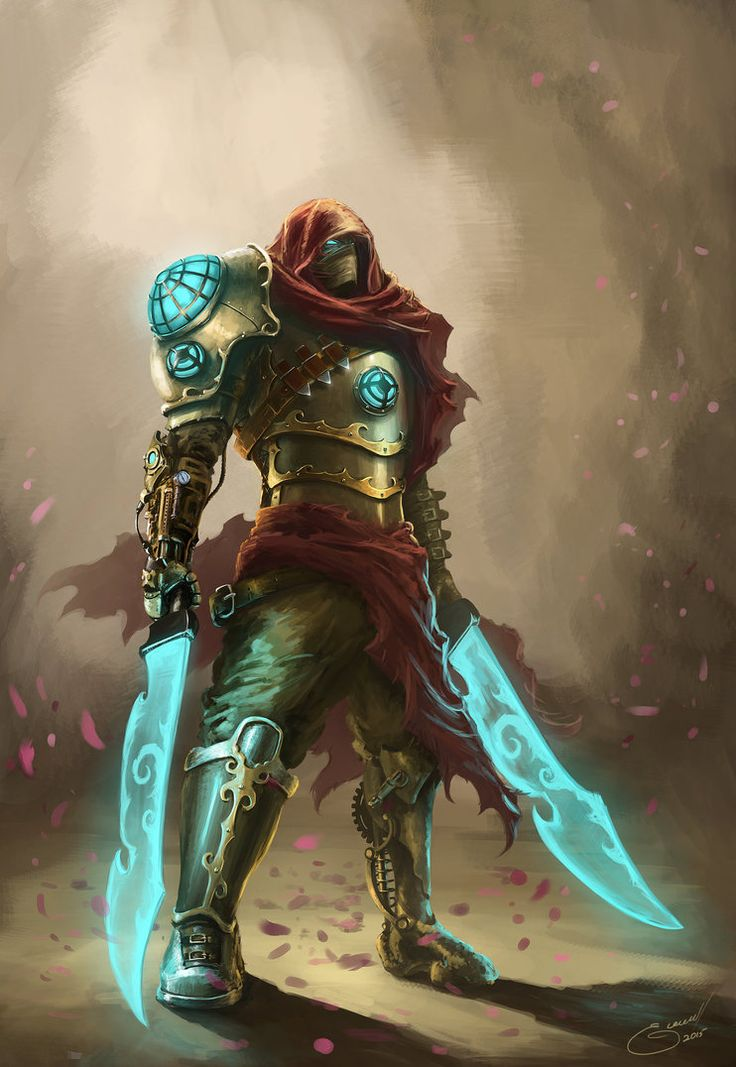
\includegraphics[scale=0.15]{../graphics/warrior}
    \end{minipage}
\end{frame}

\begin{frame}{Story}
    \begin{itemize}
        \item Heavier in beginning/end
        \item References throughout
        \item Character development
    \end{itemize}
\end{frame}

\begin{frame}{Inspiration}
    \begin{itemize}
         \item Baten Kaitos
         \item Early Final Fantasy
         \item Grain War
    \end{itemize}
\end{frame}

% TODO: add more game intro

\begin{frame}[standout]
    \Huge
    Demo
\end{frame}

\begin{frame}[standout]
    \Huge
    Post-Mortem
\end{frame}

% For Post-Mortem, maybe we have a 'general' section and one for each of our
% sub-sections? E.g. story/narration for David, music/sound for Jacob, etc.
% -- David

\begin{frame}{General}
    % first attempt at 'general' section
    \begin{itemize}
        \item GameMaker
        % I can talk about this next point based on my own code -- David
        \item Well-designed features
        \item PhotoShop
    \end{itemize}
\end{frame}

\begin{frame}{Story \& Narration}
    \begin{itemize}
        \item Consistency
        \item Motivation
        \item Characters
        \item Dialogue
    \end{itemize}
\end{frame}

\begin{frame}{Music \& Sound}
    \begin{itemize}
        \item Contrasting Music
        \item Mood Setting
        \item Identifiable Sound Effects
        \item Abundant Sound Effects
    \end{itemize}
\end{frame}

\begin{frame}[standout]
    \Huge
    Questions?
\end{frame}

\end{document}
